\FloatBarrier
\newSec[Result]{Auswertung}{2}


Aus der Berechnung der Position in z-Richtung im Vergleich mit den gemessenen Daten (siehe \refImg{fig:FlightPos}) lässt sich zeigen, dass der Ansatz grundsätzlich korrekt gewählt wurde.\\
Da die dieser Auswertung zugrundeliegenden Daten mittel der \textit{Hover}-Funkationalität der \Ar\ (siehe \refCap{parrotTopicsCMD}) aufgezeichnet wurden, ist lediglich eine geringe Abweichung in x- und y-Richtung zu erwarten. Diese kann lediglich durch die empirische Erkenntnisse, nicht durch gelegbare Daten, untermauert werden.
Im Zuge dieser \Arbeit\ konnte keine Begründung für die in \refImg{fig:FlightPos} ersichtlichen Abweichungen der Position in x- und y-Richtung vom lokalen Nullpunkt gefunden werden. Da auch eine sehr geringe Kalibrierung der \CodeClass{PoseBuildable} durchgeführte wird (vgl. \refImg{fig:FlightPoseVel}), ist davon auszugehen, dass die Abweichungen eine tiefergehende Begründung verlangen. Auch der Aufruf der \CodeMeth{reset()} für die beiden Ausrichtungen nach Änderungen der StatusID zu dem Wert 3 (\textit{Flying}) oder dem Wert 4 (\textit{Hovering}) konnte den Verlauf der berechneten Position in der horizontalen Ebene nicht zu einem zufriedenstellenden Ergebnis führen.

\begin{figure}[ht!]
\vspace{0.25cm}
\begin{center}
\fbox{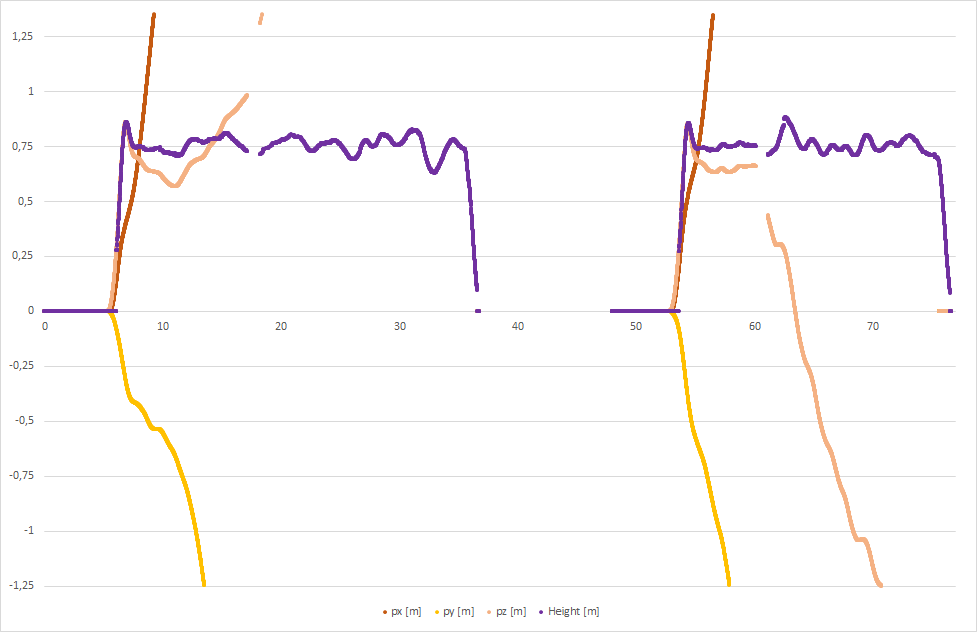
\includegraphics[width=12cm]{Pictures/TestFlight Position Med1 Avg1 Off50 Calib1.png}}
\caption{Testflug Signalverarbeitung: Aufarbeitung $a_z$}
\label{fig:FlightPos}
\end{center}

\vspace{0.25cm}
\refImgShort{fig:FlightPos} zeigt die von dem eingesetzten Programm errechneten Position des \Quad[s] \Ar\ und als Vergleichswert die vom Ultraschall-Sensor gemessenen Abstand zum Untergrund.
\end{figure}

Unter der Annahme, dass das Programm zur Berechnung der Pose korrekt implementiert wurde, kann abgeleitet werden, dass die in der \Ar\ verbauten Initialsensoren in Verbindung mit der Diskretisierung der gemessenen Werte eine Abweichung der berechneten Pose von der tatsächlichen Pose zu erwarten ist.
Diese Abweichung kann als Unsicherheit \bzw\ Wahrscheinlichkeitsverteilung in die berechnete Pose aufgenommen werden.






